The following demonstrates the calculation of output loss associated with the default using the growth accounting approach proposed by \citet{zarazaga-12}.

Following \citet{zarazaga-12}, assume that the production function follows the form $y_t = h^\alpha_t k^{1-\alpha}_t$ where $y_t$ denotes output, $k_t$ denotes physical capital, and $h_t$ denotes employment.
This implies that by the relationship $\frac{y_t}{h_t} = \left( \frac{k_t}{y_t} \right)^{\frac{1-\alpha}{\alpha}}$. If the capital-output ratio before the default episode $\kappa_b =\frac{k_b}{y_b}$ falls to $\kappa_a = \frac{k_{a}}{y_a}$ after the default episode, the output per worker would be
$\Delta = \left[\left(\frac{\kappa_a}{\kappa_b} \right)^{\frac{1-\alpha}{\alpha}} -1\right]\times 100$ percent higher.
If we ascribe all the observed decrease to the sovereign default, we conclude that the output loss is on average $\frac{\Delta}{2} \%$ per worker during the period.
Note that $\left(\frac{\kappa_a}{\kappa_b} \right)^{\frac{1-\alpha}{\alpha}} -1 > 0$ if and only if $\kappa_a > \kappa_b$. This implies that there is an output loss only if the capital-output-ratio decreases. As argued in \citet{zarazaga-12}, the output loss is associated with a trough in the capital-output-ratio.

Using data from the Penn World Table, the annually capital-output ratio is calculated by dividing the capital stock at current PPPs (variable \emph{cn}) by the output-side real GDP at current PPPs (variable \emph{cgdpo}), both in million 2017 U.S. dollar.

In the case of Sri Lanka, capital-output ratio associated with the three default episodes (2005, 2012, 2017) recorded in the BoC-BoE Sovereign Default Database all increase, even for the consecutive years, as shown in Figure \ref{fig: sri-lanka-ky}. It is therefore unreasonable to attribute all the variations of the output to the sovereign default episodes.

For the case of Pakistan's biggest default in 1999, according to previous calibration, $\alpha=$ 0.4, which implies that by the relationship $\frac{y_t}{h_t} = \left( \frac{k_t}{y_t} \right)^{\frac{3}{2}}$.
The capital-output-ratio did not immediately fall after the crisis, but instead reached to 1.43 in 2003. It fell to about 1.347 in 2005, and slowly reached 1.6 in 2009, as shown in Figure \ref{fig: pakistan-ky}.
If $\frac{k_t}{y_t}$ had not fallen from 1.43 to 1.347 between 2003 to 2005, the output per worker would have been $ \left[\left(\frac{1.43}{1.347} \right)^{\frac{3}{2}} -1\right]\times 100$, approximately 9.84\% higher. Thus on average, the output per worker turned out to be $4.9\%$ lower if we ascribe all the fall in capital-to-output ratio to the default in 1999. Hence, we conclude that the output cost of the default for Pakistan in 1999 is 5\% per year per worker.


\begin{figure}[t]
    \centering
    \begin{subfigure}[position]{0.49\textwidth}
        \centering
        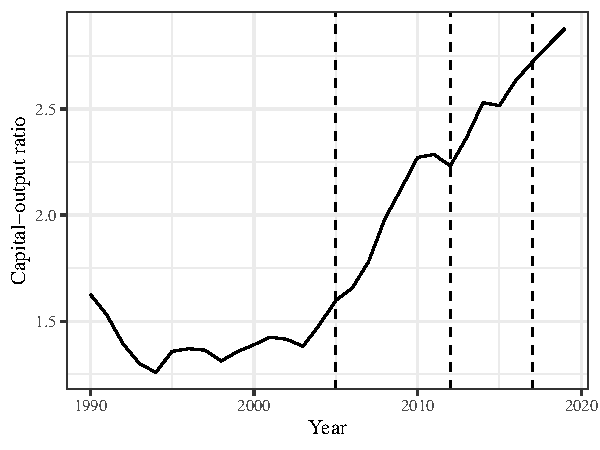
\includegraphics[width=\textwidth]{fig/sri_lanka_output_loss.pdf}
        \caption{Sri Lanka}
        \label{fig: sri-lanka-ky}
    \end{subfigure}
    \begin{subfigure}[position]{0.49\textwidth}
        \centering
        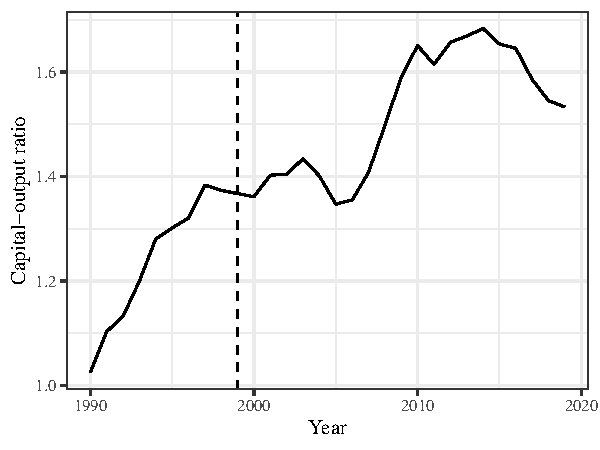
\includegraphics[width = \textwidth]{fig/pakistan_output_loss.pdf}
        \caption{Pakistan}
        \label{fig: pakistan-ky}
    \end{subfigure}
    \caption{Capital-Output Ratio, 1990 to 2020}
    \label{fig: LAK-PAK-ky}
    \floatfoot{Source: Penn World Table\\
    Note: The solid line represents the capital-output ratio for Sri Lanka and Pakistan. Default episode examined is plotted in vertical dashed lines.}
\end{figure}